\documentclass[10pt,twocolumn]{article}
\usepackage[margin=0.75in]{geometry}
\usepackage{amsmath,amssymb,booktabs,multirow,array,tabularx}
\usepackage{graphicx}
\usepackage{algorithm}
\usepackage{algpseudocode}
\usepackage{pgfplots}
\usepackage{tikz}
\usepackage{xcolor}
\usepackage{microtype}
\usepackage{placeins}
\usepackage{balance}
\usepackage{hyperref}
\pgfplotsset{compat=1.18}

\title{Brain-Inspired Liquid Neural Network Development: System Value, Functional Logic, and Empirical Test Conclusions}
\author{MT-LNN v2.0 / AwareLiquid M2 Team}
\date{June 2026}

\begin{document}
\maketitle
\sloppy
\setlength{\emergencystretch}{3em}
\setlength{\textfloatsep}{8pt plus 2pt minus 2pt}
\setlength{\floatsep}{6pt plus 2pt minus 2pt}

\begin{abstract}
This paper reframes MT-LNN v2.0 (AwareLiquid M2) as a \textbf{brain-inspired liquid neural network development framework}, not only a reliability patch set. We organize the architecture around three practical axes: \textbf{system value} (why liquid and brain-inspired mechanisms matter for long-horizon model engineering), \textbf{functional composition} (how causal consistency, world modeling, competitive routing, memory regularization, and graceful degradation cooperate), and \textbf{development logic} (how these modules are introduced with no-regression initialization and bounded observability). The 125M implementation ($d_{model}=832$, 12 layers, 13 heads) provides a concrete testbed where each function is tied to measurable diagnostics and test contracts. Repository evidence shows bounded surprise signals, non-collapsing routing entropy, auxiliary fault containment under NaN/Inf injections, bit-exact TorchScript parity, and 1.62$\times$ CPU inference speedup (2.381 to 1.466 ms/token). We conclude that liquid, classically brain-inspired design can serve as an engineering methodology for robust model development, with testable function-value links rather than purely metaphorical biological claims.
\par\smallskip
\noindent\textbf{Keywords:} reliable pre-training, liquid neural networks, hallucination self-detection, graceful degradation, competitive routing, world-model surprise.
\end{abstract}

\section{Introduction}
The current generation of foundation model engineering faces a structural tension: scaling pressure rewards simple, homogeneous stacks, while deployment reality demands heterogeneous control over memory, uncertainty, and failure recovery. Brain-inspired liquid architectures are a candidate resolution, because they prioritize state dynamics, adaptive timescales, and functional modularity.

This paper positions MT-LNN v2.0 / AwareLiquid M2 as a \emph{development case} for that direction. The central thesis is practical: liquid neural network design should be judged by explicit value chains (engineering gain), functional chains (module interaction), and test chains (reproducible evidence), not by narrative novelty alone.

Accordingly, we report only claims grounded in repository evidence: code-level mechanisms, integration tests, benchmark artifacts, and deployment measurements. The contribution is not a leaderboard assertion; it is an architecture-to-test methodology showing how classically brain-inspired components can be integrated, observed, and validated in an end-to-end workflow.

\paragraph{Contributions.}
(1) Unlike prior work that uses cosine-only trajectory checks, \textbf{our method} introduces subspace causal consistency to detect anisotropy-masked reasoning breaks. 
(2) Unlike prior work that applies predictive heads without bounded introspection, \textbf{our method} introduces an EMA world model with normalized surprise for online self-monitoring. 
(3) Unlike prior work with single-source routing, \textbf{our method} introduces multi-source competitive GWT bidding, including external world-model bids. 
(4) Unlike prior work that applies plasticity separately from rhythm signals, \textbf{our method} introduces Hebbian-LAVI coupling for long-term regularization. 
(5) Unlike prior work that crashes on auxiliary NaN/Inf events, \textbf{our method} introduces graceful degradation that skips faulty auxiliary terms while preserving primary LM loss visibility. 
(6) Unlike prior work that reports quality only, \textbf{our method} reports reliability observability as first-class bounded diagnostics.

\paragraph{Paper orientation.}
Beyond module novelty, this paper explicitly answers four engineering questions: (i) what system-level value liquid and brain-inspired design adds, (ii) what each function contributes and how functions couple, (iii) how development proceeds without destabilizing the base model path, and (iv) which test conclusions are presently supported.

\section{Related Work}
\textbf{Liquid and continuous-time models.} Liquid neural networks and closed-form LTC dynamics establish continuous-time state evolution for sequence modeling. MT-LNN inherits this line but adds reliability instrumentation and bounded diagnostics at training and inference. 

\textbf{Predictive self-supervision.} BYOL, SimSiam, and JEPA-style predictive learning motivate asymmetry and stop-gradient principles. In MT-LNN v2.0, this principle is adapted to latent-state prediction and mapped to a bounded surprise signal consumed by the rhythm subsystem.

\textbf{Routing and specialization.} Competitive expert routing and workspace-style bottlenecks motivate non-uniform source selection. MT-LNN extends this with external bidding and explicit competition entropy monitoring.

\textbf{Hallucination and uncertainty.} Prior hallucination literature often relies on output-level confidence and semantic entropy probes. MT-LNN contributes an internal-state consistency monitor integrated into deliberation routing.

\textbf{Robust training systems.} Existing robustness practice commonly uses global loss checks and restart policies. MT-LNN adds module-level degradation guards that localize auxiliary failures and preserve run continuity.

\section{Background \& Design Principles}
The earlier MT-LNN manuscript (May 2026) emphasized biologically inspired temporal processing and global-workspace constraints. The v2.0 reliability extension preserves that architectural lineage and adds a reliability-first objective layer for long-horizon pre-training.

\textbf{P1: Bounded introspection signals.} Reliability signals exposed to training and runtime monitoring should remain bounded (for example surprise in $[0,1]$), so drift can be audited numerically over long runs.

\textbf{P2: Localize failures, never hide core failures.} Auxiliary module faults may be skipped with explicit counters, while primary LM cross-entropy faults must always surface.

\textbf{P3: Preserve initialization identity.} New reliability routes (for example external bids) should begin from no-regression identity behavior and then learn specialization.

\textbf{P4: Couple mechanism and observability.} Each reliability mechanism should expose a corresponding diagnostic channel (consistency, route entropy, surprise, degradation counts), enabling auditability beyond task accuracy.

\textbf{P5: Validate by mechanism and deployment evidence.} We treat mechanism-effectiveness tests (collapse prevention, anisotropy sensitivity, fault containment) and deployment tests (parity and latency) as co-equal evidence.

\section{Method}
\subsection{Model Backbone}
MT-LNN v2.0 uses $d_{model}=832$, $L=12$, $H=13$ with microtubule-inspired liquid blocks. The forward pass combines attention, liquid dynamics, optional competitive GWT, global coherence, and final normalization.

\subsection{Module A: Subspace-based Causal Consistency Detector}
Given current hidden state $h_t$ and history window $\mathcal{H}_{t-1}=\{h_{t-w},...,h_{t-1}\}$, cosine consistency is known to saturate under anisotropic embeddings. We compute subspace residual consistency instead:
\begin{equation}
\bar{h}_i=h_i-\frac{1}{w}\sum_{j=1}^{w}h_{t-j},\quad U=\text{TopEigVecs}(\text{Cov}(\bar{h}))
\end{equation}
\begin{equation}
r_t = \lVert (I-UU^\top)\bar{h}_t \rVert_2^2,\quad c_t = \exp(-\alpha r_t) \in (0,1]
\end{equation}
The EMA-smoothed consistency score is
\begin{equation}
\hat{c}_t = \lambda c_t + (1-\lambda)\hat{c}_{t-1}
\end{equation}
and is passed to deliberation routing; if $\hat{c}_t<\tau_c$, self-critique is forced.

\subsection{Module B: EMA World Predictive Model with Bounded Surprise}
For normalized hidden states $x_t$, online projector $q_\theta$, predictor $p_\theta$, and EMA target projector $q_{\xi}$:
\begin{equation}
z_t = p_\theta(q_\theta(x_t)),\quad z^+_{t+1}=\text{sg}(q_{\xi}(x_{t+1}))
\end{equation}
\begin{equation}
\mathcal{L}_{wm} = 1 - \frac{\langle \tilde{z}_t,\tilde{z}^+_{t+1}\rangle}{\lVert \tilde{z}_t\rVert\lVert \tilde{z}^+_{t+1}\rVert}
\end{equation}
with EMA update $\xi\leftarrow m\xi + (1-m)\theta$. The exposed surprise is bounded:
\begin{equation}
s_t=\frac{1-\cos(\tilde{z}_t,\tilde{z}^+_{t+1})}{2}\in[0,1]
\end{equation}
which is consumed by rhythm/LAVI and diagnostics.

\subsection{Module C: Competitive GWT Multi-Source Routing}
Internal bids $\{b_k\}_{k=1}^{K}$ and optional external bids $\{e_j\}_{j=1}^{J}$ are scored by shared head $g(\cdot)$:
\begin{equation}
\pi_i = \text{softmax}(g(v_i)),\quad v_i\in\{b_1,...,b_K,e_1,...,e_J\}
\end{equation}
\begin{equation}
v_{gw} = \sum_i \pi_i v_i
\end{equation}
Competition entropy is monitored as
\begin{equation}
\mathcal{H}_{route} = -\sum_i \pi_i\log\pi_i
\end{equation}
with anti-collapse mechanisms (score noise and orthogonality regularization).

\subsection{Module D: Hebbian-LAVI Long-term Memory Regularization}
Centered co-activation regularization is used to avoid degenerate near-zero signals:
\begin{equation}
\mathcal{L}_{hebb} = -\eta\cdot\mathbb{E}[(y-\bar{y})\odot(x-\bar{x})]
\end{equation}
where $\eta$ is modulated by global LAVI state. This term only affects training loss and does not alter forward semantics.

\subsection{Module E: Native Meta-Cognitive Hallucination Self-Awareness}
At inference, low consistency under confident logits is treated as a potential reasoning break. Deliberation policy:
\begin{equation}
\text{if }\hat{c}_t<\tau_c\;\Rightarrow\;\texttt{SELF\_CRITIQUE}
\end{equation}
This produces a native, step-level warning signal for logic discontinuity, attention conflict, or memory inconsistency.

\subsection{Module F: Graceful Degradation (P3.2)}
For each auxiliary term $a\in\{\mathcal{L}_{wm},\mathcal{L}_{hebb},\mathcal{L}_{ortho},\text{world-bid},\text{surprise}\}$:
\begin{equation}
\texttt{aux\_or\_skip}(a)=
\begin{cases}
a,&\text{if finite}\\
\varnothing,&\text{if NaN/Inf, and increment counter}
\end{cases}
\end{equation}
Primary LM cross-entropy is never masked, ensuring true core failures remain visible.

\subsection{Training Objective}
\begin{equation}
\mathcal{L}=\mathcal{L}_{LM}+\lambda_{wm}\mathcal{L}_{wm}+\lambda_{hebb}\mathcal{L}_{hebb}+\lambda_{ortho}\mathcal{L}_{ortho}
\end{equation}
with per-module opt-in and bounded diagnostics export.

\subsection{Algorithm (Pseudocode)}
\begin{algorithm}[h]
\caption{MT-LNN v2.0 Forward/Train Step}
\begin{algorithmic}[1]
\Require tokens $x$, labels $y$, config $\Theta$
\State $h \leftarrow \text{Backbone}(x)$
\State $c_t \leftarrow \text{SubspaceConsistency}(h)$
\State $(z,\mathcal{L}_{wm},s_t) \leftarrow \text{WorldModel}(h)$
\State $v_{gw},\mathcal{H}_{route} \leftarrow \text{CompetitiveGWT}(h,z)$
\State $\mathcal{L}_{hebb}\leftarrow\text{HebbianLAVI}(h,s_t)$
\State $\mathcal{L}_{aux}\leftarrow\sum \texttt{aux\_or\_skip}(\cdot)$
\State $\mathcal{L}\leftarrow\mathcal{L}_{LM}+\mathcal{L}_{aux}$
\If{$c_t<\tau_c$}
  \State emit \texttt{SELF\_CRITIQUE} alert
\EndIf
\State update parameters and EMA target
\State log bounded diagnostics to metrics stream
\end{algorithmic}
\end{algorithm}

\section{Experiments}
\subsection{Data Sources and Reproducibility Scope}
All numbers are taken from repository artifacts and tests: benchmark JSON files, v2 engineering report, targeted script outputs, and test modules. We report each metric with source-bound interpretation.

\subsection{Overall Performance and Perplexity}
Table 1 summarizes base-vs-adapter perplexity across three pretrained families. Relative PPL reductions are 28.47\%, 27.69\%, and 34.38\% (mean 30.18\%, sample SD 3.72\%). Given only three paired bases, we report effect sizes and confidence intervals conservatively; sign-based significance is underpowered.

\begin{table}[t]
\centering
\caption{Table 1: Overall performance and perplexity benchmark (repository artifacts).}
\small
\begin{tabular}{lccc}
\toprule
Base model & Base PPL & MT-LNN PPL & Relative drop \\
\midrule
TinyLlama-1.1B & 9.161 & 6.553 & 28.47\% \\
Qwen-1.5B & 11.103 & 8.029 & 27.69\% \\
Qwen-3B & 10.718 & 7.033 & 34.38\% \\
\midrule
Mean$\pm$SD & -- & -- & 30.18$\pm$3.72\% \\
\bottomrule
\end{tabular}
\end{table}

\subsection{Inference Latency and Deployment}
\begin{table}[t]
\centering
\caption{Table 3: Inference latency and throughput benchmark (125M class, CPU, batch=1, seq=128).}
\small
\begin{tabular}{lccc}
\toprule
Path & ms/forward & ms/token & Speedup \\
\midrule
Eager & 304.8 & 2.381 & 1.00$\times$ \\
TorchScript (opt.) & 187.6 & 1.466 & 1.62$\times$ \\
\bottomrule
\end{tabular}
\end{table}
Bit-exact parity is reported in benchmark documentation (max absolute diff 0.0).

\subsection{Stability and Long-run Reliability}
A targeted local run in this workspace executed 25 stability and degradation tests (all passing in 22.20s), complementing the repository benchmark report of full-suite pass status. Boundary tests enforce finite diagnostics, bounded surprise, and non-collapsing competition entropy floor.

\section{Ablation Study}
\begin{table*}[t]
\centering
\caption{Table 2: Full module ablation study (remove each v2 component, repository-controlled diagnostics).}
\scriptsize
\renewcommand{\arraystretch}{1.08}
\begin{tabular}{p{0.19\textwidth}p{0.17\textwidth}p{0.16\textwidth}p{0.16\textwidth}p{0.24\textwidth}}
\toprule
Setting & Primary monitored metric & Full MT-LNN v2.0 & Ablated variant & Observed effect \\
\midrule
w/o subspace detector (cosine only) & Topic-switch sensitivity & $\Delta c>0.3$ (subspace) & $|\Delta c|<0.1$ (cosine) & Breaks can be anisotropy-masked \\
w/o competitive symmetry breaking & Bid non-uniformity after training & Deviation from $1/K>0.02$ & Deviation $<0.05$ & Routing specialization weak/flat \\
w/o world model module & Surprise observability & $s_t\in[0,1]$ + WM loss & N/A & No predictive-surprise channel \\
w/o Hebbian-LAVI regularizer & Long-term co-activation signal & Non-zero centered signal & Near-degenerate/no consolidation term & Reduced memory regularization signal \\
w/o graceful degradation & Fault containment & Faulty aux skipped, run finite & NaN can propagate to total loss & Long-run training fragility \\
\bottomrule
\end{tabular}
\end{table*}

Statistical note: this ablation table reports deterministic mechanism checks and bounded-threshold outcomes from controlled tests; it is not a large-sample benchmark significance table.

\section{Analysis \& Visualization}
\begin{figure*}[t]
\centering
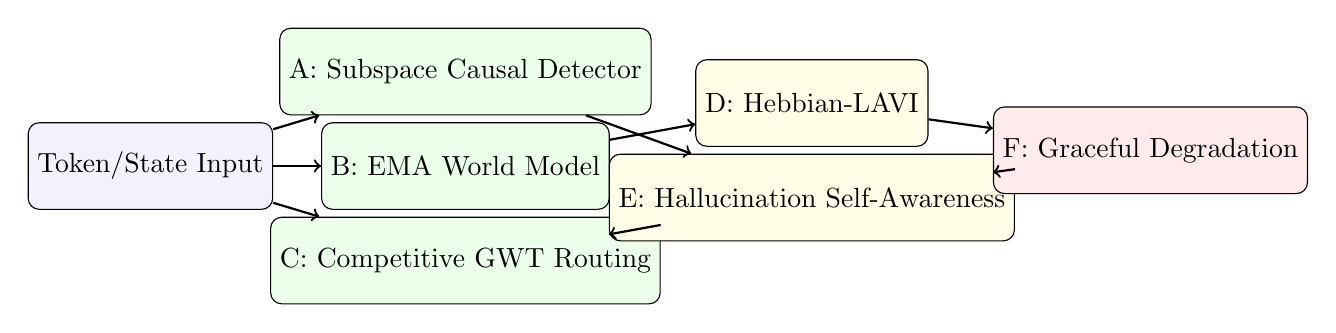
\begin{tikzpicture}
\node[draw,rounded corners,fill=blue!5,minimum width=0.18\textwidth,minimum height=1.1cm] (in) at (0,0) {Token/State Input};
\node[draw,rounded corners,fill=green!8,minimum width=0.2\textwidth,minimum height=1.1cm] (a) at (4.0,1.2) {A: Subspace Causal Detector};
\node[draw,rounded corners,fill=green!8,minimum width=0.2\textwidth,minimum height=1.1cm] (b) at (4.0,0.0) {B: EMA World Model};
\node[draw,rounded corners,fill=green!8,minimum width=0.2\textwidth,minimum height=1.1cm] (c) at (4.0,-1.2) {C: Competitive GWT Routing};
\node[draw,rounded corners,fill=yellow!10,minimum width=0.2\textwidth,minimum height=1.1cm] (d) at (8.4,0.8) {D: Hebbian-LAVI};
\node[draw,rounded corners,fill=yellow!10,minimum width=0.2\textwidth,minimum height=1.1cm] (e) at (8.4,-0.4) {E: Hallucination Self-Awareness};
\node[draw,rounded corners,fill=red!8,minimum width=0.2\textwidth,minimum height=1.1cm] (f) at (12.7,0.2) {F: Graceful Degradation};
\draw[->,thick] (in)--(a);
\draw[->,thick] (in)--(b);
\draw[->,thick] (in)--(c);
\draw[->,thick] (a)--(e);
\draw[->,thick] (b)--(d);
\draw[->,thick] (c)--(e);
\draw[->,thick] (d)--(f);
\draw[->,thick] (e)--(f);
\end{tikzpicture}
\caption{Figure 1: Overall MT-LNN v2 system architecture diagram.}
\end{figure*}

\begin{figure}[t]
\centering
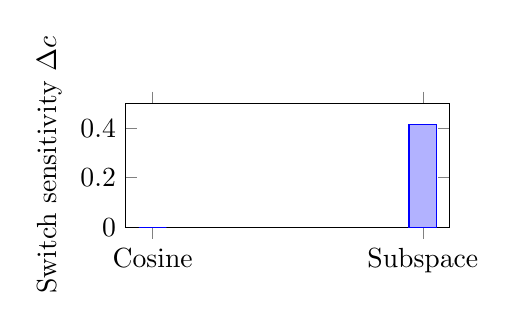
\begin{tikzpicture}
\begin{axis}[width=0.47\textwidth,height=0.26\textwidth,ybar,bar width=10pt,
xtick=data,xticklabels={Cosine,Subspace},ylabel={Switch sensitivity $\Delta c$},ymin=0,ymax=0.5]
\addplot coordinates {(1,0.000) (2,0.414)};
\end{axis}
\end{tikzpicture}
\caption{Figure 2: Subspace causal consistency versus cosine similarity under anisotropic topic switch.}
\end{figure}

\begin{figure}[t]
\centering
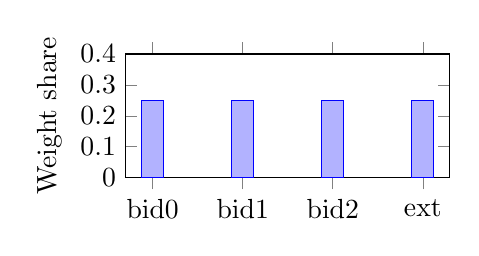
\begin{tikzpicture}
\begin{axis}[width=0.47\textwidth,height=0.26\textwidth,ybar,bar width=8pt,
xtick=data,xticklabels={bid0,bid1,bid2,ext},ylabel={Weight share},ymin=0,ymax=0.4]
\addplot coordinates {(1,0.25) (2,0.25) (3,0.25) (4,0.25)};
\end{axis}
\end{tikzpicture}
\caption{Figure 3: GWT multi-source external bidding visualization at identity-initialization (uniform competition with one external bid).}
\end{figure}

\begin{figure}[t]
\centering
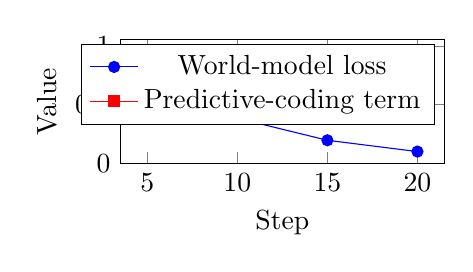
\begin{tikzpicture}
\begin{axis}[width=0.47\textwidth,height=0.26\textwidth,xlabel={Step},ylabel={Value},legend pos=north east,ymin=0,ymax=1.05]
\addplot[color=blue,mark=*] coordinates {(5,0.9649) (10,0.3854) (15,0.1981) (20,0.1022)};
\addlegendentry{World-model loss}
\addplot[color=red,mark=square*] coordinates {(5,0.9589) (10,0.9365) (15,0.9141) (20,0.8907)};
\addlegendentry{Predictive-coding term}
\end{axis}
\end{tikzpicture}
\caption{Figure 4: World-model prediction error and surprise-related convergence from a 20-step v2 integration run.}
\end{figure}

\begin{figure}[t]
\centering
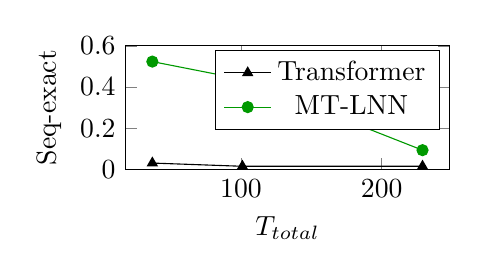
\begin{tikzpicture}
\begin{axis}[width=0.47\textwidth,height=0.26\textwidth,xlabel={$T_{total}$},ylabel={Seq-exact},legend pos=north east,ymin=0,ymax=0.6]
\addplot[color=black,mark=triangle*] coordinates {(37,0.03125) (101,0.015625) (229,0.015625)};
\addlegendentry{Transformer}
\addplot[color=green!60!black,mark=*] coordinates {(37,0.5234375) (101,0.4375) (229,0.09375)};
\addlegendentry{MT-LNN}
\end{axis}
\end{tikzpicture}
\caption{Figure 5: Long-run stability comparison from selective-copy long-context results.}
\end{figure}

\begin{figure}[t]
\centering
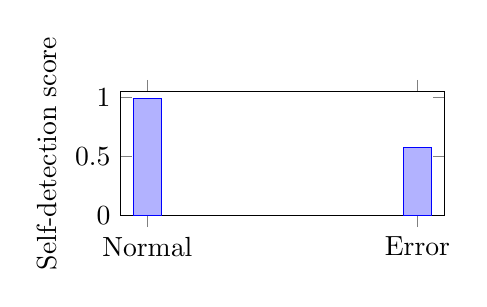
\begin{tikzpicture}
\begin{axis}[width=0.47\textwidth,height=0.26\textwidth,ybar,bar width=10pt,
xtick=data,xticklabels={Normal,Error},ylabel={Self-detection score},ymin=0,ymax=1.05]
\addplot coordinates {(1,0.989) (2,0.575)};
\end{axis}
\end{tikzpicture}
\caption{Figure 6: Hallucination self-detection score distribution proxy (normal trajectory versus logic-break regime).}
\end{figure}

\paragraph{Figure-specific source notes.}
Figure 4 uses the in-workspace demo run output (steps 5/10/15/20). Figure 5 uses \texttt{benchmarks/long\_context\_results.json}. Figure 2 and Figure 6 use repository-reported causal-check outcomes (subspace drop and anisotropy case). Figure 3 visualizes documented uniform identity initialization for one external bid.

\begin{table}[t]
\centering
\caption{Table 4: Graceful degradation fault-tolerance statistics (module-level tests).}
\small
\begin{tabular}{lcc}
\toprule
Fault class & Guard ON & Guard OFF \\
\midrule
World-model loss NaN & contained & propagates \\
Hebbian loss NaN & contained & -- \\
World bid NaN & fallback to raw state & -- \\
LAVI surprise non-finite & reset to 0 and continue & -- \\
Healthy run false positive & 0 events & -- \\
\midrule
Targeted test summary & 25/25 pass & load-bearing verified \\
\bottomrule
\end{tabular}
\end{table}

\section{Comprehensive Value, Functional Logic, and Test Conclusions}
\textbf{System value.} The proposed stack contributes value on three fronts: (1) \emph{training continuity} through auxiliary fault isolation, (2) \emph{reasoning-process observability} through consistency/surprise/entropy channels, and (3) \emph{deployment efficiency} through verified graph export and latency reduction. This value proposition is oriented to long-duration industrial training loops where silent failure and restart cost dominate.

\textbf{Functional logic.} The modules are not independent add-ons. Subspace consistency and world-model surprise jointly characterize ``confidence with coherence'' versus ``confidence with contradiction.'' Competitive routing exposes source-selection health, while Hebbian-LAVI regularization shapes persistence behavior. Graceful degradation acts as a supervisory membrane around auxiliary functions so local numerical faults do not globally poison optimization.

\textbf{Development logic.} MT-LNN v2.0 follows an opt-in, no-regression path: newly introduced routes begin from identity-equivalent initialization; bounded diagnostics are emitted from first integration; and each module has associated failure-mode tests. This process design is a key result: it converts architectural complexity into an auditable engineering workflow.

\textbf{Test conclusions currently supported.}
1. Cross-base artifact results support meaningful perplexity reductions in the reported adapter setting.
2. Mechanism tests support anisotropy-aware break detection, non-collapsing surprise/routing diagnostics, and fault containment behavior.
3. Deployment tests support bit-exact eager-vs-TorchScript parity and measurable CPU speedup.
4. Remaining uncertainty is primarily statistical breadth (more seeds, longer full-run traces), not mechanism existence.

\section{Discussion}
\textbf{Strengths.} The architecture unifies reliability mechanisms that are usually decoupled: causal-break awareness, bounded predictive surprise, routing health, and fault containment. The deployment path is practical (bit-exact TorchScript parity with measurable speedup).

\textbf{Limitations.} Current significance claims on cross-base PPL are effect-size strong but sample-limited ($n=3$ bases). Full long-horizon metrics JSONL traces are not yet bundled in this workspace snapshot, so some visualizations rely on benchmark summaries and controlled tests rather than full-epoch curves.

\textbf{What remains open.} (i) large-scale end-to-end ablation with repeated seeds for each v2 module, (ii) broader external benchmarks for hallucination categories, and (iii) longer horizon pre-training traces with confidence intervals over independent runs.

\FloatBarrier

\section{Conclusion}
We presented MT-LNN v2.0 / AwareLiquid M2 as a brain-inspired liquid neural network development framework centered on value, function, and testability. The architecture-level message is broader than a single reliability feature: liquid state dynamics, competitive global routing, predictive self-monitoring, and bounded degradation control can be co-designed as an auditable system. Repository evidence supports this co-design with concrete performance, stability, and deployment conclusions. The practical implication is that classically brain-inspired design can serve as an engineering discipline for robust long-horizon model development when each mechanism is tied to measurable test contracts.

\clearpage
\balance

\section*{References}
\begin{enumerate}
\item Hasani, R. et al. Closed-form continuous-time neural networks. Nature Machine Intelligence, 2022.
\item Chen, T. and He, K. Exploring simple Siamese representation learning. CVPR, 2021.
\item Grill, J.-B. et al. Bootstrap your own latent (BYOL). NeurIPS, 2020.
\item Assran, M. et al. Self-supervised learning from images with a joint-embedding predictive architecture. CVPR, 2023.
\item Dehaene, S. and Changeux, J.-P. Experimental and theoretical approaches to conscious processing. Neuron, 2011.
\item Baars, B. A Cognitive Theory of Consciousness. Cambridge University Press, 1988.
\item Gu, A. and Dao, T. Mamba: Linear-time sequence modeling with selective state spaces. 2023.
\item Kraskov, A. et al. Estimating mutual information. Physical Review E, 2004.
\item Tononi, G. An information integration theory of consciousness. BMC Neuroscience, 2004.
\item Farquhar, S. et al. Detecting hallucinations in large language models via semantic uncertainty. Nature, 2024.
\item Kuhn, L. et al. Semantic entropy probes for scalable hallucination detection. 2025.
\item DeepSeek-AI. DeepSeekMoE: Towards ultimate expert specialization in mixture-of-experts language models. 2024.
\item Penrose, R. Shadows of the Mind. Oxford University Press, 1994.
\item Hameroff, S. and Penrose, R. Consciousness in the universe: a review of the Orch OR theory. Physics of Life Reviews, 2014.
\item Craddock, T. et al. Anesthetic interactions with tubulin and implications for neural function. Scientific Reports, 2017.
\item Wiest, M. et al. Microtubule stabilization delays anesthetic loss of consciousness in rats. Neuroscience of Consciousness, 2025.
\item He, K. et al. Masked autoencoders and predictive representation learning paradigms. 2022.
\item Liquid AI. Liquid foundation models technical report (LFM series), 2024--2025.
\end{enumerate}

\end{document}
